\chapter{Lecture 13}

%--- 信息 ----
\begin{center}
    讲师:王立威 \qquad
    课程时间:25.May.20th \qquad 
    笔记:25.June.9th
\end{center}

\bigskip

首先完成了信道编码定理的证明,放在了前一节. 下面介绍Fisher信息和Cram​​ér-Rao不等式. 

动机和来源是无偏估计. (若学过统计学可跳过)
\begin{definition}[无偏估计]
    我们(往往独立同分布地)采样了一组样本点$X=(X_1,X_2,\dots, X_n)$,设其密度函数为$f(\cdot;\te)$(其中$\te$是我们要估计的参数),那么有 
    \[
    f(x;\te) = \prod_{i=1}^n f(X_i; \te)
    \]
    
    现在使用这些样本点得到$\te$的一个估计$\hat{\te} = \phi(X_1,\dots, X_n)$. 如果满足$\E[\hat{\te}] = \te$则称$\hat{\te}$是$\te$的\textbf{无偏估计}(unbiased estimation).
\end{definition} 

在正式定义Fisher信息之前先要引入得分函数的定义. 
\begin{definition}[得分函数]
    \textbf{得分函数}(score function)是指 
    \[
    S(X;\te) := \del{}{\te} \ln f(X;\te)
    \]
\end{definition}

\begin{proposition}
    得分函数满足$\E[S(X;\te)] = 0$
\end{proposition}
\begin{proof}
    根据定义 
    \begin{align*}
        \E[S(X;\te)] & = \int S(x;\te) f(x;\te) \dx \\
        & = \int \del{}{\te} \ln f(x;\te) f(x;\te) \\
        & = \int \del{f(x;\te)}{\te} \dfrac{1}{f(x;\te)} f(x;\te) \dx \\ 
        & = \int \del{f(x;\te)}{\te} \dx \\
        & = \del{}{\te}\int f(x;\te) \dx = \del{}{\te} \ 1 = 0
    \end{align*}
\end{proof} 

现在可以定义Fisher信息了
\begin{definition}[Fisher信息]
    对于$X,\te$,定义其Fisher信息(information)为 
    \[
    I(\te) := \var(S(X;\te)) = \E[S^2(X;\te)]
    \]
\end{definition}

\begin{proposition}
    $I(\te) = -\E\left[
        \del{^2}{\te^2} \ln f(X;\te)
    \right] = -\displaystyle\int \del{^2}{\te^2} \ln f(x;\te) f(x;\te) \dx$
\end{proposition}
\begin{proof}
    \begin{align*}
       \E\left[
        \del{^2}{\te^2} \ln f(X;\te)
    \right] & =\int \del{^2}{\te^2} \ln f(x;\te) f(x;\te) \dx \\
    & = \int \del{}{\te} \left(
        \dfrac{\nabla_\te f(x;\te)}{f(x;\te)}
    \right) f(x;\te) \dx \\
    & = \int \dfrac{\nabla^2_\te f(x;\te)\cdot f(x;\te) - (\nabla_\te f(x;\te))^2}{f^2(x;\te)} f(x;\te) \dx \\
    & = \int \nabla^2_\te f(x;\te) \dx - \int \left(\dfrac{\nabla_\te f(x;\te)}{f(x;\te)}\right)^2 f(x;\te) \dx \\
    & = \del{^2}{\te^2} \int f(x;\te) \dx -\int \del{^2}{\te^2} \ln f(x;\te) f(x;\te) \dx \\
    & = -\E\left[
        \del{^2}{\te^2} \ln f(X;\te)
    \right]
    \end{align*}
\end{proof} 

Fisher信息的意义在衡量无偏估计最好能好到什么程度,这里的好是由方差来度量的. 也就是这里要介绍的不等式:
\begin{theorem}[Cram​​ér-Rao不等式]
    对于任意$\te$的无偏估计$\phi: X \ra \R$,我们有 
    \[
    \var(\phi(X)) \ge \dfrac{1}{I(\te)}
    \]
\end{theorem}
\begin{proof}
    证明此略.
\end{proof}

我们可以将得分函数,Fisher信息,Cramér-Rao不等式拓展到$d$维的情况:

\begin{align*}
    \del{}{\te} \ln f(X;\te) \quad & \longrightarrow \quad \nabla_\te \ln f(x;\te) \\ 
    -\E\left[
        \del{^2}{\te^2} \ln f(X;\te)
    \right]\quad & \longrightarrow \quad -\E\left[
        \nabla^2_\te \ln f(X;\te)
    \right] \\
    \var(\phi(X)) \ge \dfrac{1}{I(\te)} \quad & \longrightarrow \quad  \cov(\phi(X)) \ge \dfrac{1}{I(\te)}
\end{align*}

% \begin{figure}[H]
%     \centering
%     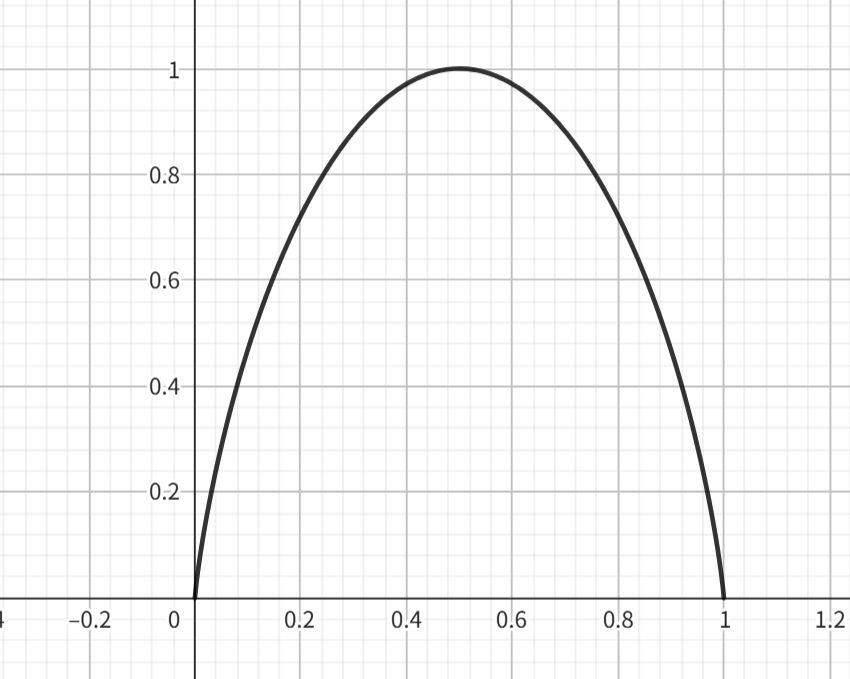
\includegraphics[width=.6\textwidth]{images/c2_1.png}
%     \caption{$H=x\log 1/x + (1-x)\log 1/(1-x)$的图像}
% \end{figure}